\subsubsection{LLNL ATDM Data \& Viz Projects: CognitiveComputing}

%%{\itshape
%%
%%	\begin{enumerate}
%%	\item Rename this file to your project WBS-projectname.tex, for example 2.3.3.01-XSDK4ECP.tex.
%%	\item Complete this template for your project.  Limit your text to two pages, not counting citations.  
%%	\item Please avoid changing the content of main.tex.  
%%	\item Put any references in a .bib file with the same root name, for example 2.3.3.01-XSDK4ECP.bib.
%%	\item Remember to include any image files you reference in your text.
%%    \item The files 2.3.3.01-XSDK4ECP.tex, 2.3.3.01-XSDK4ECP.bib and xSDK-diagram.jpeg are included as examples for your reference.  You can remove them from what you upload.
%%	\end{enumerate}
%%}

\paragraph{Overview} 

The Cognitive Simulation Project is intended to revolutionize simulation and computing efforts at LLNL.  
This effort will increase efficiencies throughout simulation and computing by creating a 
\textbf{\textit{"resource multiplier"}}, essentially using machine learning to multiplythe output of our workforce, 
simulations, and computing resources. These improvements will be achieved through broad LLNL applications that 
vary from problems that are typically solved with heuristics, as well as correcting terms in physics equations 
using machine learning techniques.

Three types of resources are targeted for creating multipliers - workforce, simulation and computing. 
Examples of creating a \textbf{\textit{workforce multiplier}} include: 1) steering of ALE simulations by predicting and 
avoiding mesh tangling, and numerical instabilities  that exist in this modeling technique. \cite{cognitive-jiang} 
2) improving workflow for combining multi-scale simulations by integrating neural networks,trained on 
high-fidelity simulation, at different scales, into continuum simulations. \cite{cognitive-Jacobs}
\textbf{\textit{Simulation multipliers}} include: 1) using machine learning techniques to create low-cost surrogate 
models to more thoroughly evaluate design space, before running more detailed simulations and 
2) improving transitional turbulence modeling using experimental data and the machine learning technique 
of backpropagation.   
\textbf{\textit{Computing multipliers}} include: 1) Using machine learning to predict when and how to offload work 
to GPUs or other accelerators, in a running simulation, to increase runtime and power efficiency and 2) recognizing 
and correcting for load imbalance in a running simulation to reduce idle processor time.
\begin{figure}[htb]
	\centering
	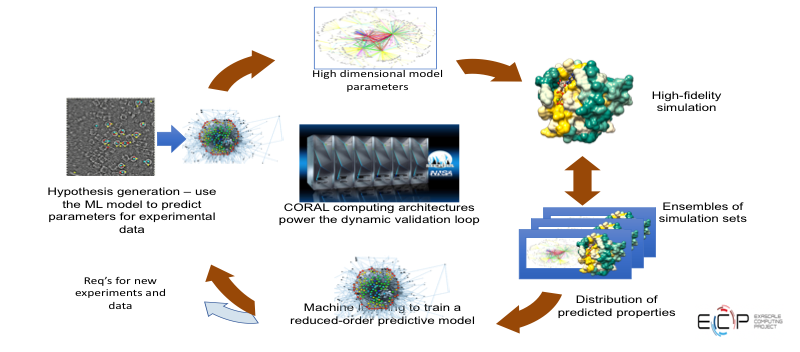
\includegraphics[width=6in]{IntegratedML}
	\caption{\label{fig:CognitiveComputing-overview} (top) Integrated machine learing, and simulation 
enables a new approach to dynamic validation of complex models. } \end{figure}

Development of this program will require continued involvement with external researchers to develop state-of-the-art, 
validated solutions.  It is imperative that we contribute to the research community through publications to maintain 
proper involvement with the external research community

\paragraph{Key Challenges}
New research areas for this work will need to address issues related to our lack of experience with machine learning 
techniques in scientific computing, and the lack of \textbf{\textit{"explainability"}} and validation of machine learning predictions. 
Although machine learning has been used in many domains, its use in scientific computing is nascent.  Many applications, 
such as producing search engine results do not need high accuracy.  High-consequence applications such as autonomous 
driving use tightly held industry algorithms.   

The external community is moving quickly, and it is vital that we collaborate with them to keep up with the latest 
technology developments.  The interdisciplinary nature of our work means that we need ML and AI expertise coupled 
with domain knowledge in the particular science and engineering.  These complementary skills are often times difficult 
to find in the same person.  High Performance Computing entails use of MPI, OpenMP, threads and other variations in 
parallel processing.  Open source ML and AI software that has been built and available via Industry are not geared 
to the HPC world, and hence we require more modification or original creations of these same types of infrastructures 
and frameworks, which are readily available and useful  for other non-scientific domains.  Difficulty in retaining 
and hiring trained experts in machine learning and AI at LLNL is a challenge, due to the competition from big name 
companies in close proximity at Silicon Valley.  Finally, we are lacking in big data, unlike Industry, where mobile 
and internet use collect massive amounts of data.  The NNSA labs tend to have reduced volumes in our data collection 
which reduces accuracy of predictions based on ML.

\paragraph{Solution Strategy}

We plan to define and address the following requirements within the next five years: 
1) application of ML techniques in ASC simulations; 2) uncertainty quantification for ML and optimization algorithms; 
3) use of ML algorithms in a distributed environment; 4) data acquisition, management, and retrieval

\paragraph{Recent Progress}

At LLNL one of the project thrusts has been material performance predictions.  Using ML data analytics we hope 
to shorten the time for certification and deployment of materials, by creating models that learn visual 
characteristics that contribute to performance.  Developing data curation, performing image analysis and 
experimental validation to corroborate results are all being actively pursued.  Initial findings show good 
predictions compared to experimental results, yet there are outliers that need further investigation.

Collaboration with University of Michigan on data-driven modeling for turbulence transition in mixing has been 
ongoing.  The work involves using Bayesian inversion plus ML to improve the Reynolds-averaged Navier-Stokes (RANS) 
model by embedding a correction function.  Early results are promising, and we have demonstrated a proof-of-concept.

Using ML for semi-automating mesh management in ALE simulations, we use supervised learning to predict mesh tanglings. 
We are proposing a novel formulation of ALE simulation resulting from deep reinforcement learning (DRL).  
The DRL4ALE project runs validation experiments for relaxation using a convolutional autoencoder network.

Learning-based predictive models:  Our need for new techniques for improving predictions in the presence of 
experimental evidence is driving this approach to integrating large-scale simulations and experiments.  This 
has resulted in the development of a cyclic system of sub-networks to engineer required performance features. 
The learning system reproduces and recovers key physics information.  The neural network performance requirements 
have led to successful predictions.  Variational extensions have equipped all output quantities with uncertainty 
measures.  Our predictive tools are prepared for statistical comparison with experiments.  Doing speculative sampling
to run our simulations may require far less data than random sampling.  That is, we only continue a simulation if we 
get unpredicted behavior.  Our initial speculative sampling experiments delivered better learned models for much less data.
  

\paragraph{Next Steps}
We intend to establish methodologies for evaluating applicability of ML techniques to our applications.  
Image classification is being done for ASC applications and a prototype capability using ML for ALE steering 
in the KULL application code will be delivered, gathering and presenting initial scaling and performance metrics.  
The Inertial Confinement Fusion (ICF) community has applications for machine learning that will also continue to be 
explored.  Evaluation on scalable frameworks for our specific use cases will also be done.

The second area is to grow greater our understanding of characteristics that make or do not make an application a good
use case. Investigation of rigorous methods for validating machine learning techniques for ASC applications will be 
performed, creating an initial measure of confidence for specific sets of data.  Finally, we will create tools to 
provide feedback to the user community about how confidence was calculated and how it can be improved.


